\documentclass[12pt]{beamer}
\usepackage{../Estilos/BeamerFC}
\usepackage{../Estilos/ColoresLatex}
\usepackage{courier}
\usepackage{listingsutf8}
\usepackage{listings}
\usepackage{xcolor}
\usepackage{textcomp}
\usepackage{color}
\definecolor{deepblue}{rgb}{0,0,0.5}
\definecolor{brown}{rgb}{0.59, 0.29, 0.0}
\definecolor{OliveGreen}{rgb}{0,0.25,0}
% \usepackage{minted}

\DeclareCaptionFont{white}{\color{white}}
\DeclareCaptionFormat{listing}{\colorbox{gray}{\parbox{0.98\textwidth}{#1#2#3}}}
\captionsetup[lstlisting]{format=listing,labelfont=white,textfont=white}
\renewcommand{\lstlistingname}{Código}


\definecolor{Code}{rgb}{0,0,0}
\definecolor{Keywords}{rgb}{255,0,0}
\definecolor{Strings}{rgb}{255,0,255}
\definecolor{Comments}{rgb}{0,0,255}
\definecolor{Numbers}{rgb}{255,128,0}

\makeatletter

\newif\iffirstchar\firstchartrue
\newif\ifstartedbyadigit
\newif\ifprecededbyequalsign

\newcommand\processletter
{%
  \ifnum\lst@mode=\lst@Pmode%
    \iffirstchar%
        \global\startedbyadigitfalse%
      \fi
      \global\firstcharfalse%
    \fi
}

\newcommand\processdigit
{%
  \ifnum\lst@mode=\lst@Pmode%
      \iffirstchar%
        \global\startedbyadigittrue%
      \fi
      \global\firstcharfalse%
  \fi
}

\lst@AddToHook{OutputOther}%
{%
  \lst@IfLastOtherOneOf{=}
    {\global\precededbyequalsigntrue}
    {}%
}

\lst@AddToHook{Output}%
{%
  \ifprecededbyequalsign%
      \ifstartedbyadigit%
        \def\lst@thestyle{\color{orange}}%
      \fi
    \fi
  \global\firstchartrue%
  \global\startedbyadigitfalse%
  \global\precededbyequalsignfalse%
}

\lstset{ 
language=Python,                % choose the language of the code
basicstyle=\footnotesize\ttfamily,       % the size of the fonts that are used for the code
numbers=left,                   % where to put the line-numbers
numberstyle=\scriptsize,      % the size of the fonts that are used for the line-numbers
stepnumber=1,                   % the step between two line-numbers. If it is 1 each line will be numbered
numbersep=5pt,                  % how far the line-numbers are from the code
backgroundcolor=\color{white},  % choose the background color. You must add \usepackage{color}
showspaces=false,               % show spaces adding particular underscores
showstringspaces=false,         % underline spaces within strings
showtabs=false,                 % show tabs within strings adding particular underscores
frame=single,   		% adds a frame around the code
tabsize=2,  		% sets default tabsize to 2 spaces
captionpos=t,   		% sets the caption-position to bottom
breaklines=true,    	% sets automatic line breaking
breakatwhitespace=false,    % sets if automatic breaks should only happen at whitespace
escapeinside={| |},  % if you want to add a comment within your code
stringstyle =\color{OliveGreen},
otherkeywords={as, np.array, np.concatenate, np.linspace, linspace, interpolate.interp1d, kind, plt.plot, .copy, np.arange, np.cos, np.pi, lw, ls, label, splrep, splev, plt.legend, loc, plt.title, plt.ylim, plt.show, sign, math.ceil, math.log, np.sqrt, np.exp, np.zeros, plt.xlabel, plt.ylabel, plt.xlim, np.identity, random, np.dot, np.outer, np.diagonal },             % Add keywords here
keywordstyle = \color{blue},
commentstyle = \color{darkcerulean},
identifierstyle = \color{black},
literate=%
         {á}{{\'a}}1
         {é}{{\'e}}1
         {í}{{\'i}}1
         {ó}{{\'o}}1
         {ú}{{\'u}}1
%
%keywordstyle=\ttb\color{deepblue}
%fancyvrb = true,
}

\lstdefinestyle{FormattedNumber}{%
    literate={0}{{\textcolor{red}{0}}}{1}%
             {1}{{\textcolor{red}{1}}}{1}%
             {2}{{\textcolor{red}{2}}}{1}%
             {3}{{\textcolor{red}{3}}}{1}%
             {4}{{\textcolor{red}{4}}}{1}%
             {5}{{\textcolor{red}{5}}}{1}%
             {6}{{\textcolor{red}{6}}}{1}%
             {7}{{\textcolor{red}{7}}}{1}%
             {8}{{\textcolor{red}{8}}}{1}%
             {9}{{\textcolor{red}{9}}}{1}%
             {.0}{{\textcolor{red}{.0}}}{2}% Following is to ensure that only periods
             {.1}{{\textcolor{red}{.1}}}{2}% followed by a digit are changed.
             {.2}{{\textcolor{red}{.2}}}{2}%
             {.3}{{\textcolor{red}{.3}}}{2}%
             {.4}{{\textcolor{red}{.4}}}{2}%
             {.5}{{\textcolor{red}{.5}}}{2}%
             {.6}{{\textcolor{red}{.6}}}{2}%
             {.7}{{\textcolor{red}{.7}}}{2}%
             {.8}{{\textcolor{red}{.8}}}{2}%
             {.9}{{\textcolor{red}{.9}}}{2}%
             {\ }{{ }}{1}% handle the space
         ,%
          %mathescape=true
          escapeinside={__}
          }



\usetheme{Warsaw}
\usecolortheme{seahorse}
%\useoutertheme{default}
\setbeamercovered{invisible}
% or whatever (possibly just delete it)
\setbeamertemplate{section in toc}[sections numbered]
\setbeamertemplate{subsection in toc}[subsections numbered]
\setbeamertemplate{subsection in toc}{\leavevmode\leftskip=3.2em\rlap{\hskip-2em\inserttocsectionnumber.\inserttocsubsectionnumber}\inserttocsubsection\par}
\setbeamercolor{section in toc}{fg=blue}
\setbeamercolor{subsection in toc}{fg=blue}
\setbeamercolor{frametitle}{fg=blue}
\setbeamertemplate{caption}[numbered]

\setbeamertemplate{footline}
\beamertemplatenavigationsymbolsempty
\setbeamertemplate{headline}{}


\makeatletter
\setbeamercolor{section in foot}{bg=gray!30, fg=black!90!orange}
\setbeamercolor{subsection in foot}{bg=blue!30}
\setbeamercolor{date in foot}{bg=black}
\setbeamertemplate{footline}
{
  \leavevmode%
  \hbox{%
  \begin{beamercolorbox}[wd=.333333\paperwidth,ht=2.25ex,dp=1ex,center]{section in foot}%
    \usebeamerfont{section in foot} \insertsection
  \end{beamercolorbox}%
  \begin{beamercolorbox}[wd=.333333\paperwidth,ht=2.25ex,dp=1ex,center]{subsection in foot}%
    \usebeamerfont{subsection in foot}  \insertsubsection
  \end{beamercolorbox}%
  \begin{beamercolorbox}[wd=.333333\paperwidth,ht=2.25ex,dp=1ex,right]{date in head/foot}%
    \usebeamerfont{date in head/foot} \insertshortdate{} \hspace*{2em}
    \insertframenumber{} / \inserttotalframenumber \hspace*{2ex} 
  \end{beamercolorbox}}%
  \vskip0pt%
}
\makeatother

\makeatletter
\patchcmd{\beamer@sectionintoc}{\vskip1.5em}{\vskip0.8em}{}{}
\makeatother

%\newlength{\depthofsumsign}
%\setlength{\depthofsumsign}{\depthof{$\sum$}}
% \newcommand{\nsum}[1][1.4]{% only for \displaystyle
%     \mathop{%
%         \raisebox
%             {-#1\depthofsumsign+1\depthofsumsign}
%             {\scalebox
%                 {#1}
%                 {$\displaystyle\sum$}%
%             }
%     }
% }
\def\scaleint#1{\vcenter{\hbox{\scaleto[3ex]{\displaystyle\int}{#1}}}}
\def\scaleoint#1{\vcenter{\hbox{\scaleto[3ex]{\displaystyle\oint}{#1}}}}
\def\bs{\mkern-12mu}

% \usefonttheme{serif}

\title{\large{Tema 1 - La mecánica de una bicicleta}}
\author{M. en C. Gustavo Contreras Mayén}
\date{ }

\begin{document}
\maketitle

\section*{Contenido}
\frame[allowframebreaks]{\frametitle{Contenido} \tableofcontents[currentsection, hideallsubsections]}

\section{La mecánica de una bicicleta}
\frame{\tableofcontents[currentsection, hideothersubsections]}
\subsection{Un modelo equivocado}

\begin{frame}
\frametitle{Una fuente de error}
Se considera un tipo de error cuando consideramos un modelo que no está en congruencia con la física.
\\
\bigskip
\pause
Veamos el siguiente ejemplo.
\end{frame}
\begin{frame}
\frametitle{Planteando el problema}
La bicicleta es una forma muy eficiente de transporte, este es un hecho bien conocido por cualquier persona que la utliza.
\\
\bigskip
\pause
Nuestro objetivo en este ejercicio es comprender los factores que determinan la velocidad máxima de una bicicleta y estimar la velocidad de un caso real.
\end{frame}

\subsection{Primera aproximación}

\begin{frame}
\frametitle{Primera aproximación}
Comenzaremos haciendo \textocolor{ao}{caso omiso de la fricción}; \pause tendremos que añadirlo al final, por supuesto, pero debemos primero entender cómo lidiar con el caso más simple y sin fricción.
\end{frame}
\begin{frame}
\frametitle{Usando la mecánica de Newton}
La ecuación de movimiento corresponde a la segunda ley de Newton, que escribimos de la forma:
\pause
\begin{equation}
\dv{v}{t} = \dfrac{F}{m}
\label{EqNewton2}
\end{equation}
donde $v$ es la velocidad, $m$ es la masa de la combinación de la bicicleta-conductor, $t$ es el tiempo, y $F$ es la fuerza en la bicicleta que viene del esfuerzo del conductor (en este caso vamos a suponer que la bicicleta se mueve sobre un terreno plano).
\end{frame}
\begin{frame}
\frametitle{Simplificando el sistema}
Tratar correctamente a $F$ se complica por la mecánica de la bicicleta, \pause ya que la fuerza ejercida por el ciclista se transmite a las ruedas por medio del plato, engranajes, cadena, etc.
\begin{figure}
    \centering
    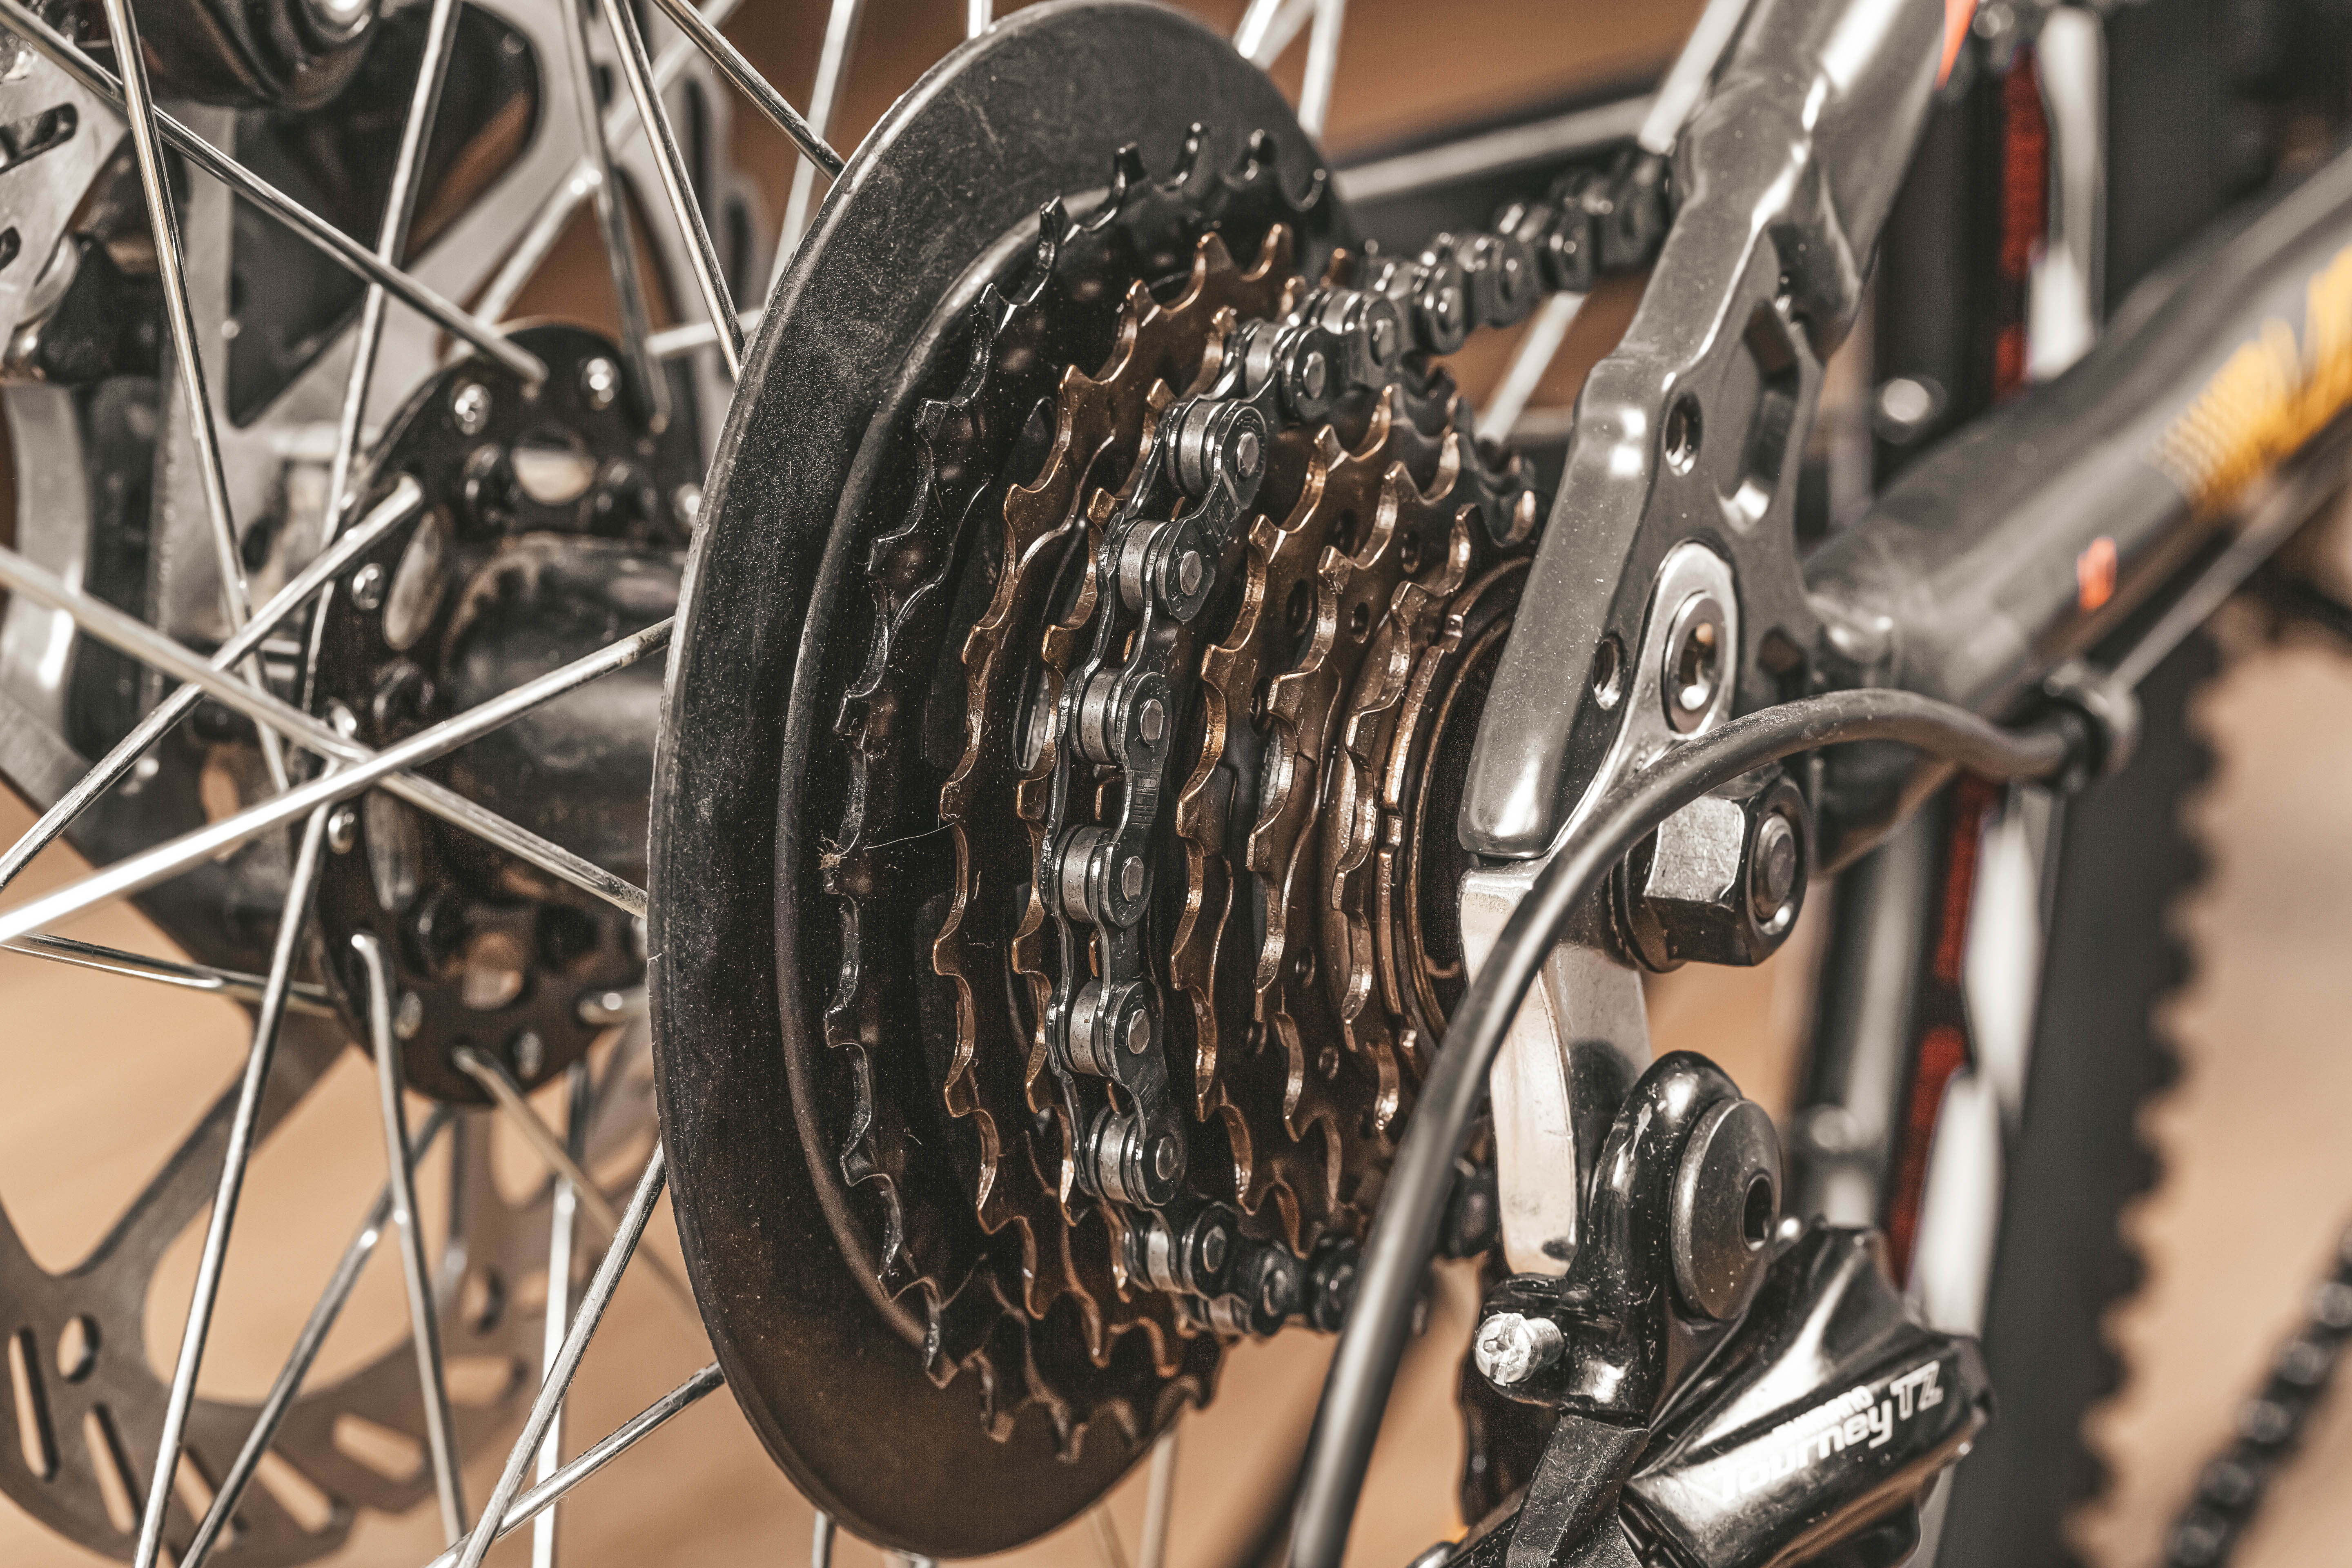
\includegraphics[scale=0.1]{Imagenes/Bicicleta_Engranes.jpg}
\end{figure}
\end{frame}
\begin{frame}
\frametitle{Simplificando el sistema}
Esto hace que sea muy difícil obtener una expresión exacta para $F$.
\end{frame}
\begin{frame}
\frametitle{Abordando el problema con otro enfoque}
Sin embargo, hay otra manera de abordar este problema que evita la necesidad de conocer la fuerza.
\\
\bigskip
\pause
Este enfoque alternativo implica la formulación del problema en términos de la potencia generada por el ciclista.
\end{frame}
\begin{frame}
\frametitle{Abordando el problema con otro enfoque}
Estudios fisiológicos de ciclistas de carreras han demostrado que estos atletas son capaces de producir una potencia de salida de aproximadamente $\SI{400}{\watt}$ durante largos períodos de tiempo ($\sim \SI{1}{\hour}$)
\begin{figure}
    \centering
    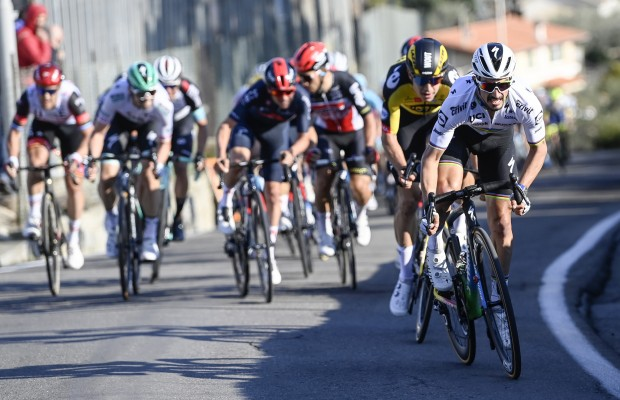
\includegraphics[scale=0.375]{Imagenes/Bicicleta_Tour.jpg}
\end{figure}
\end{frame}
\begin{frame}
\frametitle{Reescribiendo la ecuación de movimiento}
Usando las ideas de trabajo-energía podemos reescribir (\ref{EqNewton2}) como:
\pause
\begin{equation}
\dv{E}{t} = P
\label{EqPotencia}
\end{equation}
donde $E$ es la energía total, $P$ es la potencia de salida del ciclista.
\end{frame}
\begin{frame}
\frametitle{Relación entre la potencia y acelaración}
Para un trayecto plano la energía es totalmente cinética, es decir, $E = \frac{1}{2} m v^{2}$, y $\dv*{E}{t} = m \, v (\dv*{v}{t})$, usando esto en la ec. (\ref{EqPotencia}), resulta:
\pause
\begin{equation}
\dv{v}{t} = \dfrac{P}{m \, v}
\label{EqPotenciavel}
\end{equation}
\end{frame}
\begin{frame}
\frametitle{Cuando la potencia es constante}
Si $P$ es una constante, la ecuación (\ref{EqPotenciavel}), se puede resolver de manera analítica, rearreglando términos:
\pause
\begin{equation}
\scaleint{6ex}_{\bs v_{0}}^{v} v^{\prime} \dd{v^{\prime}} = \scaleint{6ex}_{\bs 0}^{t} \dfrac{P}{m} \dd{t^{\prime}}
\label{EqIntegral}
\end{equation}
donde $v_{0}$ es la velocidad de la bicicleta en $t = 0$.
\end{frame}
\begin{frame}
\frametitle{Abordando el problema con otro enfoque}
Integrando ambos lados de la ecuación y resolviendo para $v$, tenemos que:
\pause
\begin{equation}\label{Eqvres}
v = \sqrt{v_{0}^{2} + 2 \, P \dfrac{t}{m}}
\end{equation}
\end{frame}
\begin{frame}
\frametitle{¿La solución es consistente con la física?}
Si bien esta es la solución correcta de la ecuación de movimiento (\ref{EqPotenciavel}), nuestro trabajo no concluye aquí: \pause ya que predice que \textocolor{lava}{la velocidad se incrementará sin límite para tiempos muy largos}.
\\
\bigskip
\pause
Este resultado no es congruente con la física que conocemos.
\end{frame}

\subsection{Segunda aproximación}

\begin{frame}
\frametitle{Segunda aproximación}
Vamos a corregir este resultado: cuando se generaliza el modelo se debe de \textocolor{ao}{incluir el efecto de la resistencia del aire}.
\\
\bigskip
\pause
El nuevo término que vamos a añadir a la ecuación de movimiento nos obliga a desarrollar una solución numérica, así que con eso en mente se considera un tratamiento numérico de la ec. (\ref{EqPotenciavel}).
\end{frame}
\begin{frame}
\frametitle{Haciendo diferencias}
Comenzamos con la forma de diferencias finitas para la derivada de la velocidad:
\pause
\begin{equation}
\dv{v}{t} \simeq \dfrac{v_{i + 1} - v_{i}}{\Delta t}
\label{Eqderivada}
\end{equation}
donde asumimos que $\Delta t$ es paso discreto pequeño, y $v_{i}$ es la velocidad al tiempo $t_{i} \equiv i \Delta t$
\end{frame}
\begin{frame}
\frametitle{Relación entre velocidad y potencia}
Por lo que de la ecuación (\ref{EqPotenciavel}):
\pause
\begin{equation}
v_{i + 1} = v_{i} + \dfrac{P}{m \, v_{i}} \, \Delta \, t
\label{Eqveli+1}
\end{equation}
Dada la velocidad en un tiempo $i$ (es decir, $v_{i}$), podemos usar (\ref{Eqveli+1}) para calcular un valor \textit{aproximado} de la velocidad en el siguiente paso $v_{i+1}$.
\end{frame}
\begin{frame}
\frametitle{Abordando el problema con otro enfoque}
Si conocemos la velocidad inicial $v_{0}$, podemos obtener $v_{1}$, $v_{2}$, y así sucesivamente.
\\
\bigskip
\pause
Ya contamos con suficientes elementos para proponer un código en \python{}, incluiremos una gráfica del resultado.
\end{frame}

\subsection{Codificando}

\begin{frame}[allowframebreaks, fragile]
\frametitle{Abordando el problema con otro enfoque}
\begin{lstlisting}[basicstyle=\linespread{1.2}\ttfamily\small, columns=fullflexible,escapeinside=||]
import matplotlib.pyplot as plt
from math import sqrt

t = []
v = []

dt = 1

potencia = 400
masa = 70
tmax = 200
nmax = tmax/dt

t.append(0)
v.append(4)

for i in range(int(tmax/dt)):
    ti = t[i-1] + dt
    vi = sqrt(v[i]**2 + (2 * potencia * dt)/masa)
    
    
    t.append(ti)
    v.append(vi)

plt.plot(v, "r-")
plt.xlabel("tiempo [s]")
plt.ylabel("velocidad m/s")
plt.show()
\end{lstlisting}
\end{frame}

\subsection{Primer resultado}

\begin{frame}
\frametitle{Resultado de la velocidad sin fricción}
\begin{figure}[H]
	\centering
	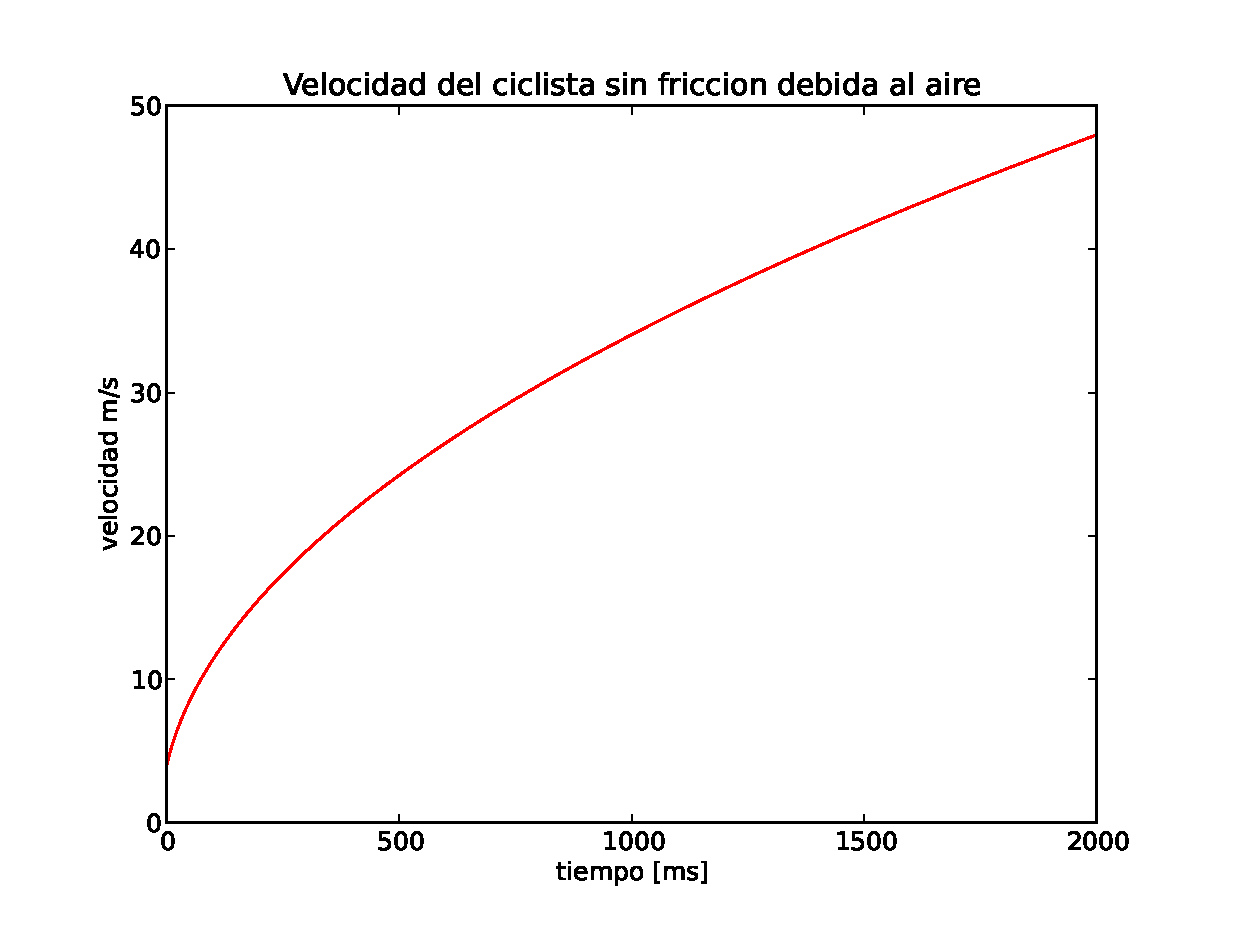
\includegraphics[scale=0.475]{Imagenes/EjerBicicleta01.eps}
\end{figure}
\end{frame}
\begin{frame}
\frametitle{Resultado ¿correcto?}
Consideremos que:
\setbeamercolor{item projected}{bg=amber,fg=black}
\setbeamertemplate{enumerate items}{%
\usebeamercolor[bg]{item projected}%
\raisebox{1.5pt}{\colorbox{bg}{\color{fg}\footnotesize\insertenumlabel}}%
}
\begin{enumerate}[<+->]
\item Hemos desarrollado un algoritmo que resuelve el problema inicial.
\item Los valores son consistentes.
\item La gráfica nos indica el comportamiento de la solución.
\end{enumerate}
\pause
Aún así: ¿debemos de considerar el problema como bien resuelto? \pause \textocolor{auburn}{No!}
\end{frame}

\subsection{Considerando la fricción del aire}

\begin{frame}
\frametitle{Segunda aproximación}
La fuerza debida a la fricción puede aproximarse de manera inicial como:
\pause
\begin{equation}
F_{a} \simeq - B_{1} \, v - B_{2} v^{2}
\label{EqFfriccion}
\end{equation}
Para velocidades muy bajas, el primer término es el que domina, y el coeficiente $B_{1}$ se puede calcular para objetos con formas sencillas.
\end{frame}
\begin{frame}
\frametitle{El tamaño del  objeto}
Para una velocidad razonable $v^{2}$ el término domina sobre los demás, pero $B_{2}$ no puede calcularse exactamente en objetos sencillos como una pelota de beisbol, menos para una bicicleta.
\end{frame}
\begin{frame}
\frametitle{Haciendo otra aproximación}
Podemos aproximar el valor de $B_{2}$ como sigue:
\\
\bigskip
\pause
Si un objeto se mueve a través de la atmósfera, debe empujar fuera del camino el aire delante de él. 
\end{frame}
\begin{frame}
\frametitle{Haciendo otra aproximación}
La masa de aire movida en el tiempo $\dd{t}$ es $m_{\text{aire}} \sim \rho A \: v \: \dd{t}$, donde $\rho$ 
es la densidad del aire y $A$ el área frontal del objeto.
\\
\bigskip
\pause
Este aire tiene una velocidad de orden $v$, y por lo tanto, su energía cinética es $E_{\text{aire}} \sim m_{\text{aire}} \: v^{2} / 2$.
\end{frame}
\begin{frame}
\frametitle{Haciendo otra aproximación}
Este es también el trabajo realizado por la fuerza de arrastre (la fuerza sobre el objeto debido a la resistencia del aire) en el tiempo $\dd{t}$, por lo $F_{a} \: \dd{t} = E_{\text{aire}}$.
\\
\bigskip
\pause
Al juntar estos resultados, encontramos que:
\pause
\begin{align*}
F_{a} \simeq - C \: \rho \: A \: v^{2}
\end{align*}
\end{frame}
\begin{frame}
\frametitle{Nueva expresión}
Incluyendo este término en la expresión para la velocidad:
\pause
\begin{equation}
v_{i+1} = v_{i} + \dfrac{P}{m \: v_{i}} \Delta \: t - \dfrac{C \: \rho \: A \: v_{i}^{2}}{m} \: \Delta \: t
\label{Eqvelifriccion}
\end{equation}
\end{frame}
\begin{frame}
\frametitle{Pasando al código}
\textbf{Ejercicio a cuenta: } Implementar el código en \python, considerando los valores $C = 0.5$ y $A=0.33$.
\\
\bigskip
\pause
De tal manera que al obtener la gráfica de la solución, debes de presentar una figura con el siguiente resultado:
\end{frame}

\subsection{Resultado consistente}

\begin{frame}
\frametitle{Velocidad en las dos aproximaciones}
\begin{figure}[H]
	\centering
	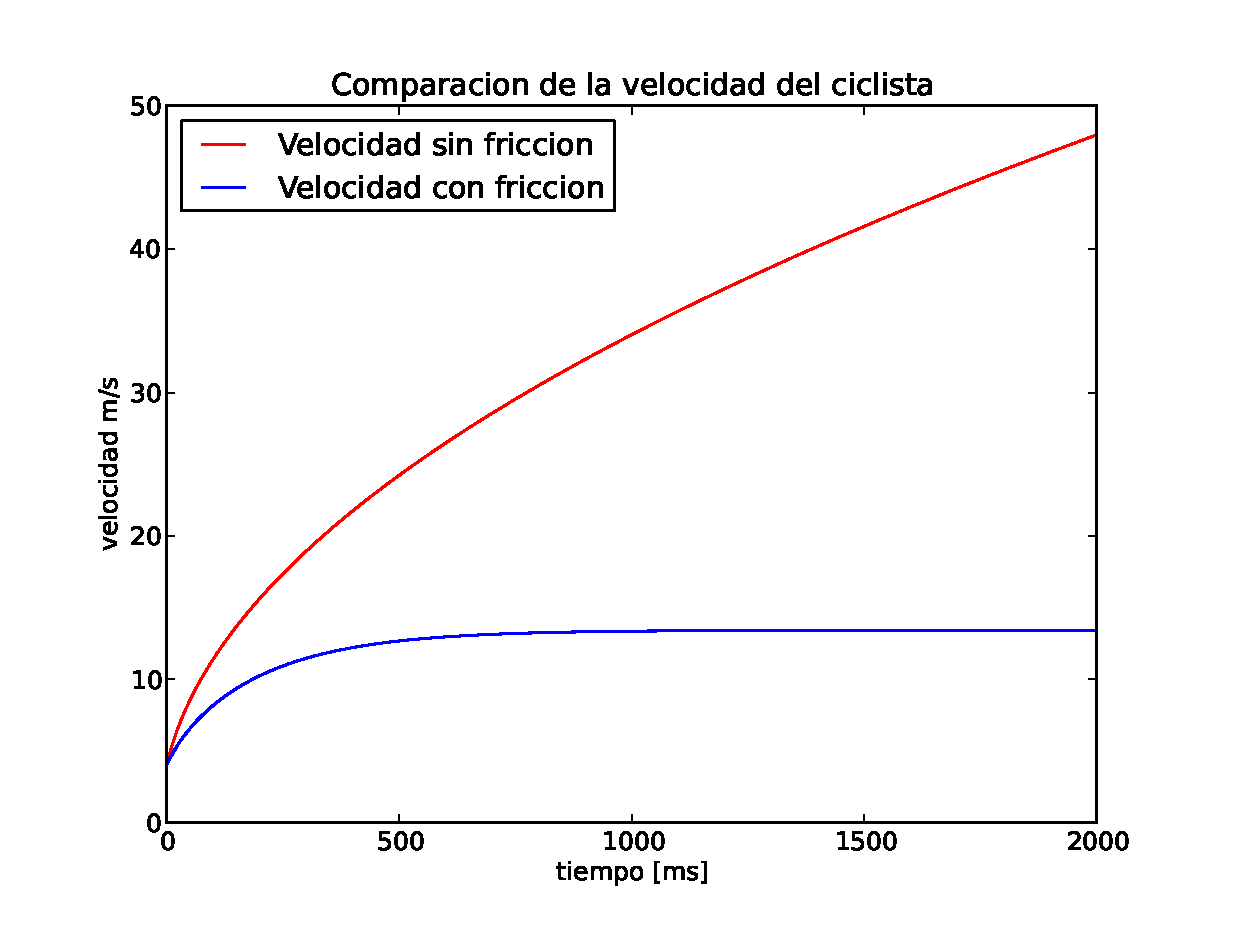
\includegraphics[scale=0.475]{Imagenes/EjerBicicleta02.eps}
\end{figure}
\end{frame}
\begin{frame}
\frametitle{Conclusión importante}
El resultado que tenemos a partir de nuestra solución numérica con la segunda aproximación, \textocolor{ao}{es más congruente con la física}.
\\
\bigskip
\pause
Nota que a pesar de tener un algoritmo que resuelve una ecuación de movimiento, nuestrto trabajo no termina con proporcionar una respuesta con el código, \pause sino que revisemos la consistencia de la solución con la física que ya manejamos.
\end{frame}
\end{document}